\subsection{Ecuación de recurrencia de primer orden}

\begin{frame}
\frametitle{\subsecname}

\begin{block}{}
	Solución general a la ecuación de recurrencia: \[ S_{n+1} = aS_n + c \qquad \qquad \forall n \in \mathds{N} \]
	Se da en dos partes:
	\begin{tabular}{cll}
		Si $a=1$, & $S_n = S_0 + nc$ & $\forall n \in \mathds{N}$\\
		Si $a\neq 1$& $S_n = a^n [S_0 - \frac{c}{1-a}] + \frac{c}{1-a}$  &$\forall n \in \mathds{N} $
		\end{tabular}
	\end{block}
\end{frame}

\subsubsection{Torre de Hanói}

\begin{frame}
%\frametitle{\subsecname}
\frametitle{Aplicación}

\begin{block}{Torres de Hanói}
	$$S_{n}=2S_{n-1}+1\quad\textit{para cada $n \geq 2$}$$
\end{block}

\begin{block}{}
	\begin{figure}
		\centering
		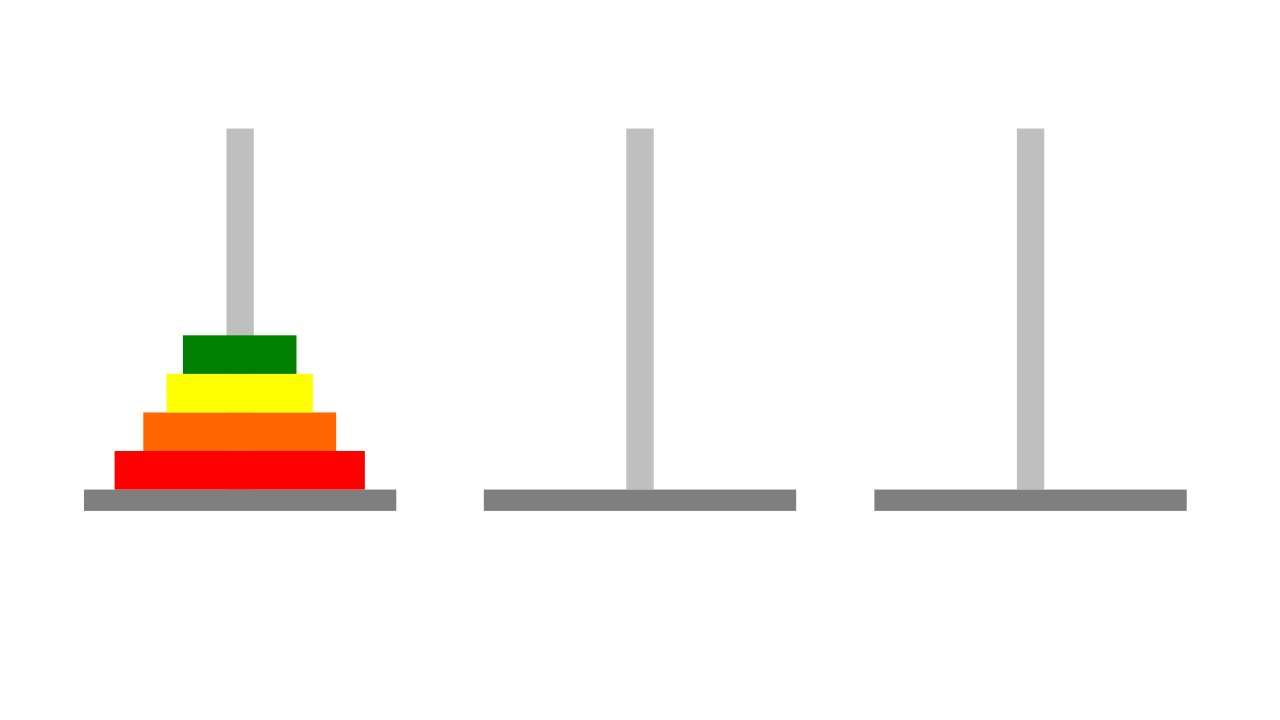
\includegraphics[scale=0.15]{torre.jpg}
	\end{figure}
\end{block}
\end{frame}

\section{Ecuaciones de recurrencia}

\begin{frame}
\frametitle{Ecuación de recurrencia de segundo orden}

\begin{block}{Teorema 1}
$S_n = A(r_1)^n + B(r_2)^n$ si $r_1 \neq r_2$, siempre que $\Delta\neq0$.
\end{block}

\begin{block}{Teorema 2}
$S_n = A(r)^n + Bn(r)^n$ si $r_1 = r_2 = r$, siempre que $\Delta=0$.
\end{block}
\end{frame}

\begin{frame}
\frametitle{Aplicación}

\begin{block}{Un modelo de cunicultura (Sucesión de Fibonacci)}
$$F_n = F_{n-1} + F_{n-2} \qquad \textit{para cada $n \geq 2$}$$
\end{block}

\begin{block}{}
	\begin{figure}
		\centering
		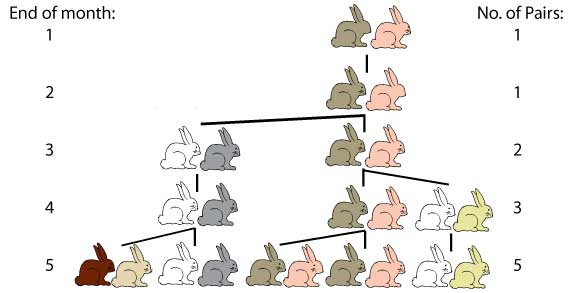
\includegraphics[scale=0.40]{conejos.jpg}
	\end{figure}
\end{block}
\end{frame}